\subsection{Abstract Factory}
Viene utilizzato per fornire la possibilità al client di creare oggetti appartenenti ad una gerarchia di prodotti, senza dover specificare le classi concrete.
\begin{figure}[ht]
    \centering
    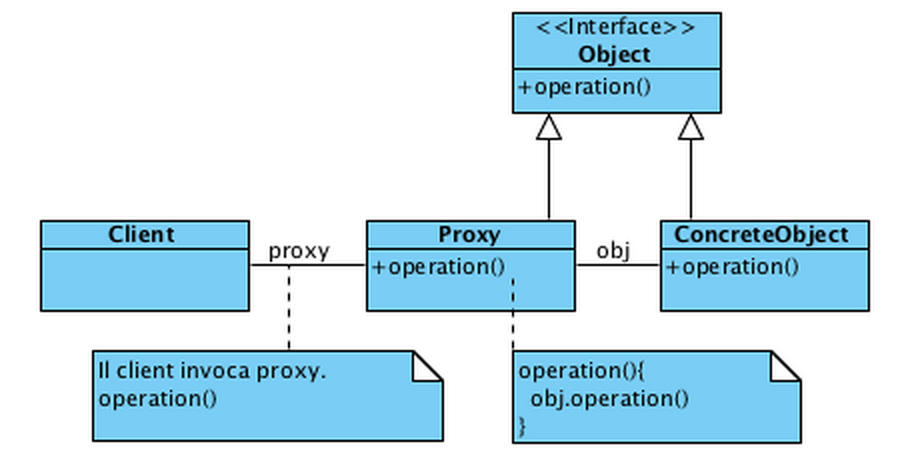
\includegraphics[width=0.8\textwidth]{immagini/proxy.png}
    \caption{Proxy}
\end{figure}
\FloatBarrier

Utilizzando questo pattern le classi client possono lavorare semplicemente con le interfacce, senza aver bisogno di conoscere i tipi concreti.
Tendenzialmente una Abstract Factory implementa un Singleton.

\subsubsection{Casi tipici}
\begin{itemize}
\item La creazione di oggetti deve essere indipendente dal sistema che li utilizza;
\item Il sistema deve poter lavorare con più famiglie degli stessi oggetti;
\item Varie famiglie di oggetti devono essere usate assieme;
\item Devono essere pubblicate delle librerie e non si vogliono mostrare i dettagli implementativi;
\item Il client non deve conoscere le classi concrete con cui lavora.
\end{itemize}